\section{Introduction}

Since the publication of RT-1 \cite{RT-1} the robotics research is undergoing a prolific period focused around foundation models. The central promise of this paradigm is the development of generalist policies that aim to achieve general-purpose embodied intelligence, capable of complex interactions within unstructured environments. This shift mirrors advancements in Machine Learning, particularly in Natural Language Processing and Computer Vision, where large pretrained models have demonstrated remarkable success.

\begin{wrapfigure}{r}{0.45\textwidth}
    \centering
    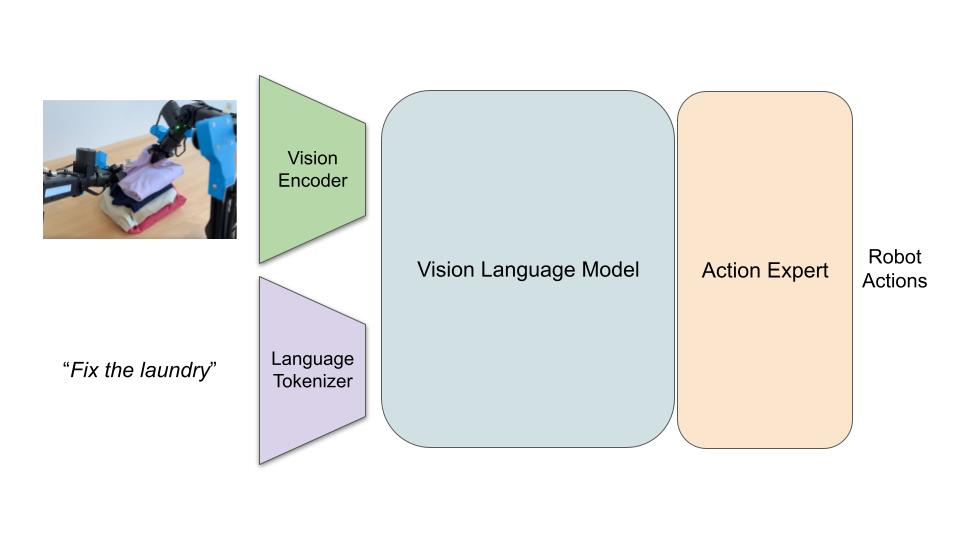
\includegraphics[width=0.45\textwidth]{images/vla.jpg}
    \caption{VLA abstraction}
    \label{fig:vla_abstraction}
    % https://docs.google.com/presentation/d/1F3-KIjQxwBtXfJAlc9_vwuBLSGuZqcXqZ7_GfxX5kYY/edit?usp=sharing
\end{wrapfigure}

Robotics foundational models, often referred to as Vision-Language-Action (VLA) models, is the name of the policies emerging from this paradigm shift. This nomenclature reflects their modality: vision and language for inputs while action as outputs (Figure \ref{fig:vla_abstraction}). Leveraging techniques such as Imitation Learning and Reinforcement Learning, these models demonstrated remarkable capabilities in dexterous manipulation across multiple tasks, offering a degree of generalization over robot embodiments and environments. The key enabler of this progress is the usage of a pretrained vision language model for initialization of the model (or part of the model), and subsequently exploit a vast and variegated robotics dataset to train the Vision Language Action Model.

\section{Goals and Objectives}
Due to the rapid pace of development in robotics foundation models, the field currently lacks established, comprehensive comparison benchmarks, particularly for complex interaction scenarios like deformable object manipulation (DOM). This makes rigorous comparison between proposed models (e.g., $\pi_0$, $Gr00t_{N1}$, $OpenVLA$) challenging. While some models like $\pi_0$ have demonstrated specific DOM tasks (Shirt/Towel/Laundry Folding), a standardized suite is needed for equitable evaluation and deeper understanding.

The primary objective of this project is to develop DOM-Bench: a standardized benchmarking suite tailored for evaluating robotics foundation models on deformable object manipulation tasks. This will provide a coherent and equitable basis for comparing model capabilities and limitations.

\subsection{Overall Goal}

This project aims to deliver:
\begin{itemize}
    \item \textbf{DOM-Bench Suite:} A well-defined set of deformable object manipulation tasks, environments, and metrics designed to evaluate robotics foundation models.
    \item \textbf{Evaluation Protocol:} A clear procedure for applying the benchmark suite to different models, including specifications for data efficiency testing.
    \item \textbf{Comparative Analysis \& Paper:} Implementation of the protocol on selected models, summarization of findings, and dissemination through a research paper.
\end{itemize}


\subsection{Specific Objectives}

To achieve the overall goal, the following specific objectives are defined:

\subsubsection{Literature Review} % Using subsubsection for better structure
Conduct a comprehensive review covering: existing robotics benchmarks, evaluation methodologies, and taxonomies, with a focus on deformable object manipulation and metrics used; Robotics foundation models (VLAs), detailing architectures, training data/recipes, and claimed capabilities relevant to manipulation.

\subsubsection{Benchmark Design (DOM-Bench)}
Propose a standardized benchmark suite (DOM-Bench) and evaluation protocol. The design will focus on providing multidimensional insights into model capabilities beyond simple task success rates.

% \paragraph{Minimum Requirements:} % Using paragraph for logical grouping within subsubsection
\begin{itemize}
    \item \textbf{Multi-Tier Task Structure:} Define tasks across tiers of increasing complexity, each with their own measurable metrics, assessing different capabilities:
        \begin{itemize}
            \item \textit{Tier 1 (Fundamentals):} Focus on evaluating core shape control and manipulation primitives using standardized objects and refined metrics.
            \item \textit{Tier 2 (Complex Interactions):} Focus on evaluating performance on tasks requiring more sophisticated interaction, multi-step execution, or tool use.
            \item \textit{Tier 3 (Foundation Model Evaluation):} Focus specifically on evaluating language understanding, reasoning, planning, and generalization capabilities inherent to foundation models when applied to DOM.
        \end{itemize}
    \item \textbf{Generalization Assessment \cite{TransferWelle}:} Systematically evaluate model generalization across key axes:
        \begin{itemize}
            \item \textit{Environments:} Define evaluation in both simulation and real-world settings (RPL lab).
            \item \textit{Tasks:} Utilize the multi-tier structure described above. (See Appendix \ref{app:task_suite} for task details).
            \item \textit{Embodiments:} Define target robot embodiments for evaluation (Minimum: SO-100; Stretch: Others available at RPL). The protocol should allow for adaptation to different embodiments where feasible.
        \end{itemize}
    \item \textbf{Data Efficiency Evaluation:} Quantify model performance relative to the amount of task-specific fine-tuning data.
        \begin{itemize}
            \item \textit{Zero-Shot Performance:} Evaluate capabilities directly using the pre-trained foundation model (0 examples).
            \item \textit{Few-Shot Performance:} Evaluate after fine-tuning on a small, standardized number of demonstrations (e.g., 10 examples, 30 examples).
        \end{itemize}
\end{itemize}

\paragraph{Stretch Goals:}
\begin{itemize}
    \item \textbf{Context Horizon Quantification:} Design specific long-horizon tasks (potentially extensions of Tier 3 tasks or dedicated scenarios) to quantitatively assess the effective context length a model can utilize for successful task completion. This involves evaluating performance degradation as task complexity and required memory increase.
    \item \textbf{Explainable AI Integration:} Incorporate methods (e.g., representational probing \cite{Probing-VLA}, attention analysis) to gain insights into the models' internal representations and decision-making processes during DOM tasks. This aims to move beyond black-box evaluation towards understanding \textit{why} models succeed or fail.
    \item \textbf{Further Tasks Expansion:} Include highly complex or nuanced tasks within the tiers (marked in Appendix \ref{app:task_suite}) that push the limits of current model capabilities (e.g., intricate knotting, delicate material handling, creative construction).
\end{itemize}

\paragraph{Protocol Definition:} Define a precise experimental protocol specifying setup, initial state randomization, number of trials, permissible interventions (if any), and data logging requirements. Reference Appendix \ref{app:task_suite} for detailed task specifications.

\subsubsection{Evaluation \& Analysis}
Implement the defined evaluation protocol using the DOM-Bench suite. Therefore, the first step is to apply the protocol to a core set of publicly available foundation models:
\begin{itemize}
    \item $\pi_0$ \cite{pi_zero}
    \item OpenVLA \cite{OpenVLA}
    \item Gr00t N1 \cite{Gr00tN1}
\end{itemize}
And a posteriori, analyze the results based on the defined metrics, focusing on comparative performance across models, tiers, generalization axes, and data efficiency levels.

\paragraph{Stretch Goals:}
Evaluation expansion can be achieved by adding additional models:
    \begin{itemize}
        \item OpenVLA-OFT \cite{OpenVLA-OFT}
        \item Octo \cite{Octo}
    \end{itemize}
Or by conducting a deeper analysis following the extension of the benchmark.


